\documentclass[border=4pt]{standalone}
\usepackage{fontspec}
\setmainfont{Times New Roman}
\setmonofont{Consolas}
\usepackage{tikz}
\usetikzlibrary{arrows.meta,positioning,shapes.geometric,calc}
\definecolor{tutorteal}{HTML}{087F7A}
\definecolor{tutorlight}{HTML}{EDF7F5}
\definecolor{tutorink}{HTML}{20323C}
\newcommand{\code}[1]{\texttt{\detokenize{#1}}}
\tikzset{box/.style={draw=tutorteal,rounded corners=2pt,fill=tutorlight,
 align=center,minimum height=10mm,text width=35mm,font=\small,inner sep=5pt},
 decision/.style={diamond,aspect=2.0,draw=tutorteal,fill=white,align=center,
 text width=23mm,font=\small,inner sep=1pt},
 flow/.style={-{Latex[length=2mm]},thick,draw=tutorink},
 optional/.style={flow,dashed}}
\begin{document}
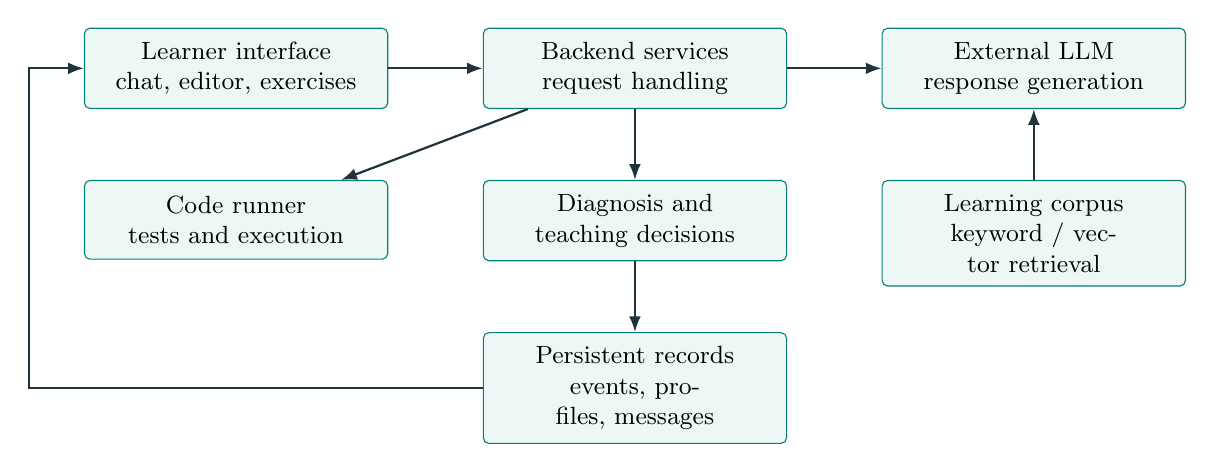
\begin{tikzpicture}[node distance=9mm and 12mm]
\node[box] (user) {Learner interface\\chat, editor, exercises};
\node[box,right=of user] (api) {Backend services\\request handling};
\node[box,right=of api] (model) {External LLM\\response generation};
\node[box,below=of user] (run) {Code runner\\tests and execution};
\node[box,below=of api] (diag) {Diagnosis and\\teaching decisions};
\node[box,below=of model] (rag) {Learning corpus\\keyword / vector retrieval};
\node[box,below=of diag] (db) {Persistent records\\events, profiles, messages};
\draw[flow] (user)--(api);
\draw[flow] (api)--(model);
\draw[flow] (api)--(diag);
\draw[flow] (api)--(run);
\draw[flow] (rag)--(model);
\draw[flow] (diag)--(db);
\draw[flow] (db.west) -- ++(-8mm,0) -| ([xshift=-7mm]user.west) -- (user.west);
\end{tikzpicture}
\end{document}
